\chapter{Stand der Wissenschaft}

\section{Funktionsweise eines CNN}\label{sec:conv}
Die Quelle für dieses Unterkapitel ist soweit nicht anders vermerkt ein Buch über \enquote{Deep Learning} \cite{CNNBook}.
Ein CNN besteht in der Regel aus mehreren Conv-Layern und einem oder mehreren Fully-Connected Layern. Die Conv-Layer sind dabei das Herzstück dieser Netzform. Eine beispielhafte Übersicht über die CNN-Architektur ist in Abbildung \ref{fig:cnn} zu sehen.


\begin{figure}[h]
  \centering
  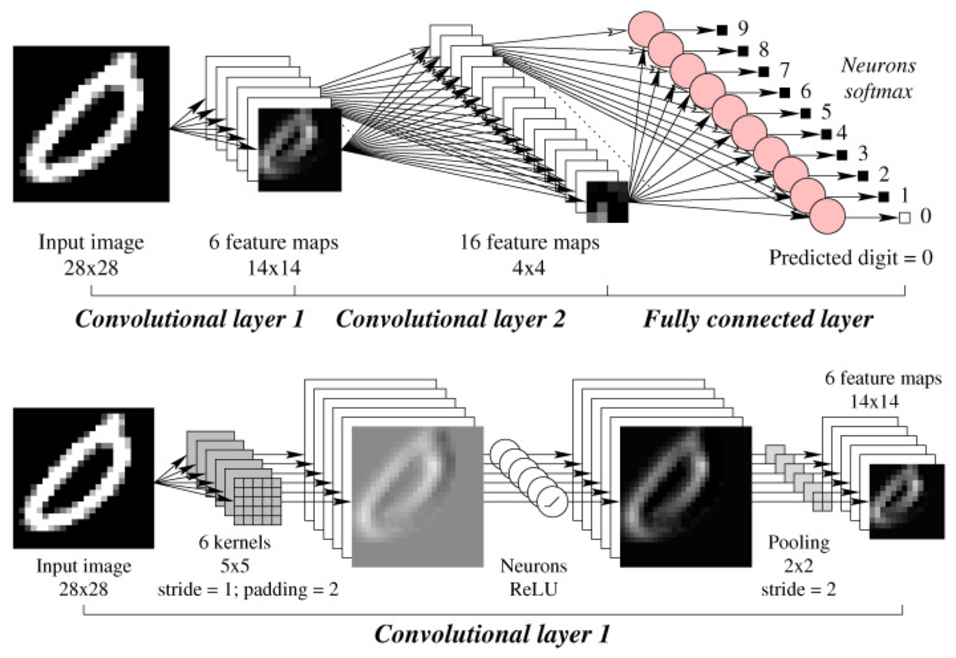
\includegraphics[width=0.75\textwidth]{images/cnn.pdf}
  \caption{Convolutional Neural Net \cite{CNNImg}}
  \label{fig:cnn}
\end{figure}


Der Unterschied zu einem \enquote{Multilayer-Perzeptron (MLP)\footnote{Die Hintergründe des MLPs und allgemein neuronaler Netzwerke werden hier nicht behandelt. Für eine Einführung in neuronale Netzwerke kann aber \cite{neural} herangezogen werden}} ist, dass bei einem MLP jede Verbindung zwischen Neuronen und die Neuronen selber ein eigenes trainierbares Gewicht haben. Ein MLP ist ein klassisches neuronales Netz, welches nur aus Fully-Connected Layern besteht. Beim CNN werden pro Schicht in einem Layer nur die Elemente der Filtermaske trainiert. Zusammen mit der viel kleineren Größe der Filter ergibt sich beim CNN im Vergleich zum MLP eine geringere Anzahl an Parametern die trainiert werden.

In Abbildung \ref{fig:cnn} ist zu sehen, dass ein CNN aus hintereinander geschalteten Conv-Layer besteht. Die Funktion der Conv-Layer wird nun näher betrachtet.

Wie in Abbildung \ref{fig:cnn} zu sehen ist, ist ein Conv-Layer die hintereinander Schaltung verschiedener Operationen:
\begin{itemize}
 \item Faltung des Eingabebildes mit dem Kernel
 \item Anwendung der Aktivierungsfunktion ReLU
 \item Pooling
\end{itemize}
Die Funktionsweise dieser Filter wird nun anhand eines Beispiels, welches in Abbildung \ref{fig:maus} zu sehen ist, erklärt.

\begin{figure}[h]
  \centering
  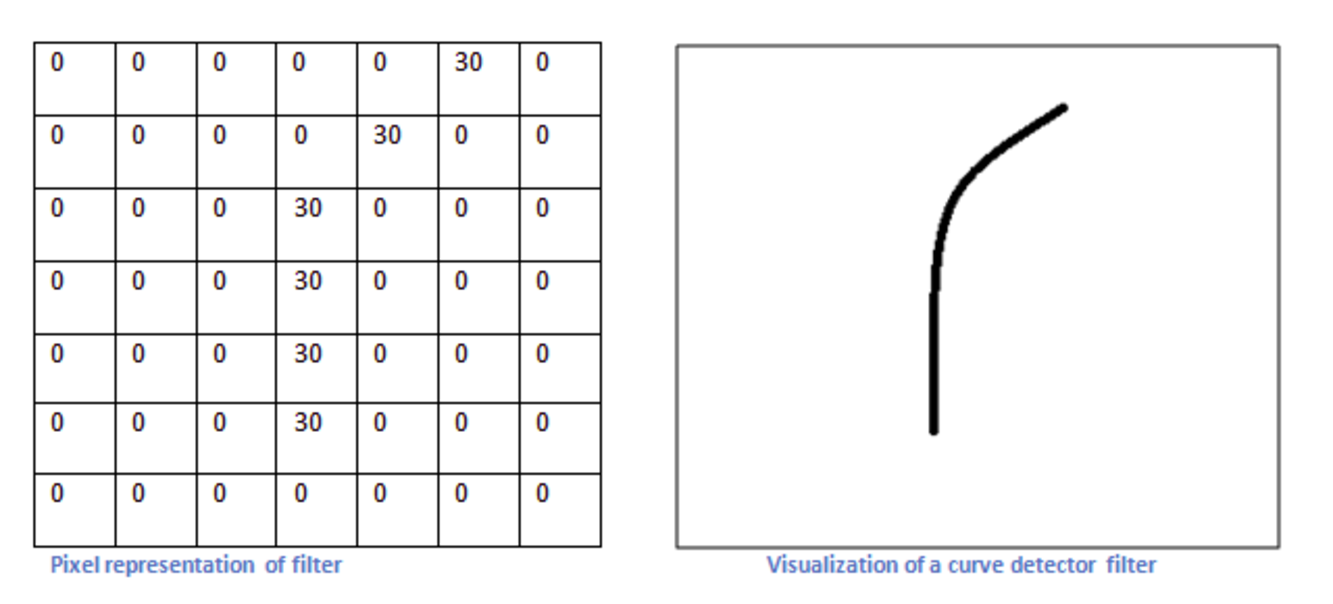
\includegraphics[width=0.5\textwidth]{images/filter.pdf}
  \caption{Filter graphische und numerische Repräsentation \cite{github}}
  \label{fig:filter}
\end{figure}

Ein Filter hat in der Regel eine Größe, die viel kleiner als das Gesamtbild ist. Die Mitte dieses Filter wird dann an jeder Bildposition aufgelegt. Nun wird aus den jeweils aufeinander liegenden Feldern ein Produkt gebildet. Die Ergebnisse der Produkte werden addiert, normiert und in der Feature Map abgespeichert. In Abbildung \ref{fig:filter} ist ein Filter, der eine gebogene Linie erkennt, zu sehen. 
Die positive Erkennung einer ähnlich gekrümmten Linie ist in Abbildung \ref{fig:maus} zu sehen. Wie eine negative Erkennung aussieht, ist in Abbildung \ref{fig:maus_n} zu sehen. 
Bei mehreren hintereinander geschalteten Conv-Layern werden die erkannten Features komplexer. So ist die Klassifikation von komplexen Mustern möglich.

Bei der Faltung des Filter mit dem Input Bild werden nur lineare Operationen verwendet. Um mit dem Netz komplexe Erkennung zu ermöglichen, benötigt es Nicht-Linearität. Diese Nicht-Linearität wird mit der Rectified Linear Unit (ReLu) erreicht. Dieses ReLu wird auf das Ergebnis der Faltung angewendet. 

\begin{figure}
    \centering
    \begin{subfigure}{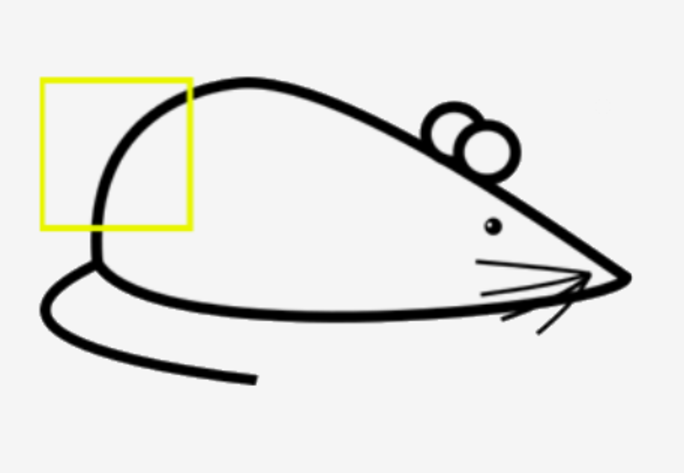
\includegraphics[width=0.25\textwidth]{images/cnn_maus.pdf}}
    \end{subfigure}
    \begin{subfigure}{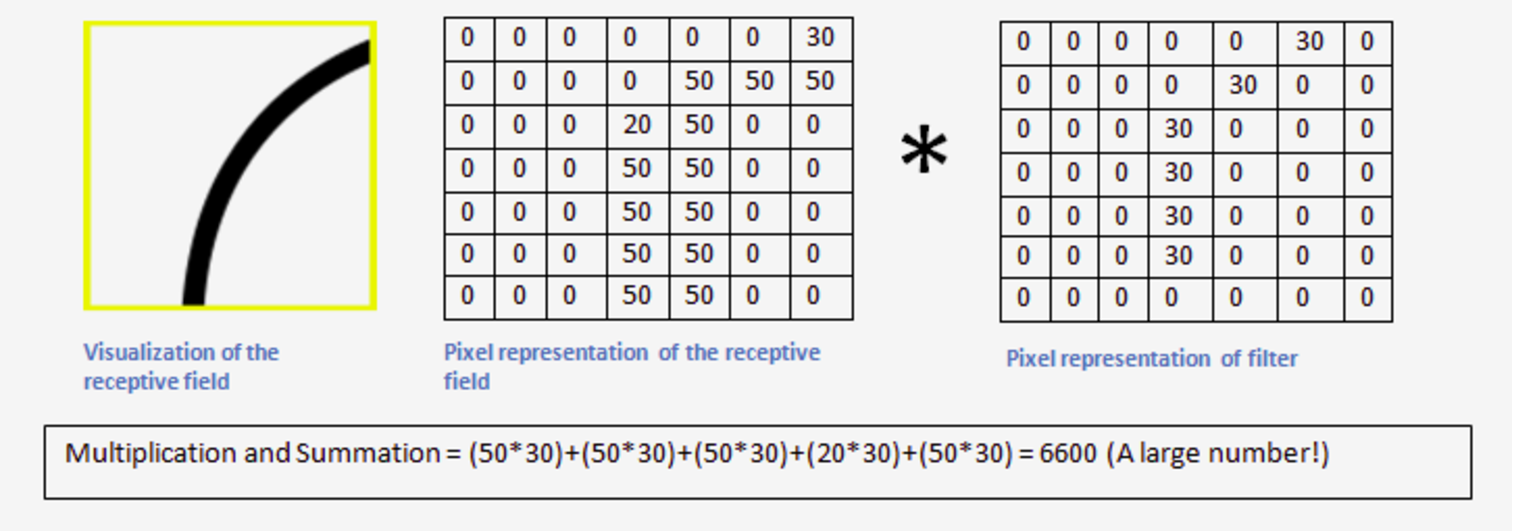
\includegraphics[width=0.5\textwidth]{images/cnn_maus_p.pdf}}
    \end{subfigure}
    \caption{positive Erkennung des Features \enquote{gebogene Linie} \cite{github}}
    \label{fig:maus}
\end{figure}

\begin{figure}[h]
  \centering
  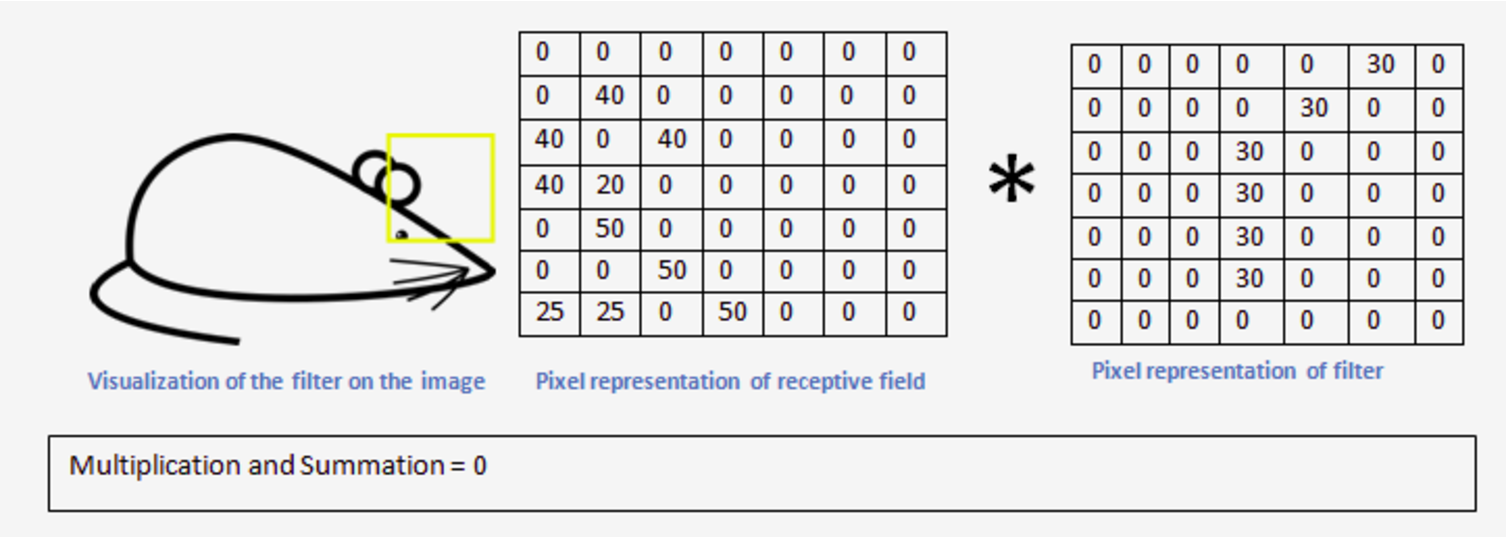
\includegraphics[width=0.5\textwidth]{images/cnn_maus_n.pdf}
  \caption{negative Erkennung des Features \enquote{gebogene Linie} \cite{github}}
  \label{fig:maus_n}
\end{figure}



Abbildung \ref{fig:cnn} beinhaltet auch noch die Begriffe Stride und Padding, welche für das Verstehen dieser Arbeit zwar nicht notwendig sind, hier der Vollständigkeit halber trotzdem erklärt werden. 

Padding löst das Problem, das entsteht, wenn der Mittelpunkt des Filters auf ein Pixel im Randbereich gelegt wird. Hier taucht das Problem auf, dass der Filter auch auf nicht vorhandenen Pixeln aufliegt und die Filteroperation hier somit nicht definiert ist. Padding setzt nun den Rand fort oder belegt diesen Rand mit einem festgelegten Wert, um dort eine gültige Filteroperation zu erzeugen. 

Stride ist der Parameter, der bestimmt um wie viele Felder der Filter nach der Anwendung verschoben werden soll. Bei größerem Stride kann die entstehende Feature-Map verkleinert werden.

Pooling ist eine Operation, die die Größe der Feature-Map verkleinert und somit Overfitting vermeidet.

Die Fully-Connected-Layer errechnen aus den Ausgängen der Convolutional-Layer, in welche Klasse ein Objekt klassifiziert werden soll.  

Die Filter, die auf die Feature Maps bzw. die Eingabebilder angewendet werden, sind trainierbar. Zusätzlich sind auch die Gewichtungen des Fully-Connected Layers trainierbar. Das heißt durch den Trainingsprozess wird versucht die Werte in der Filtermatrix und des Fully-Connected Layer so zu verändern, dass das gesamte CNN besser klassifizieren kann. Für diese Veränderung wird ein Gradientenabstiegsverfahren, welches rückwärts durch die Schichten propagiert wird, benutzt.


\section{Überblick über die gängigen Methoden}



\subsection{Suchbegriffe}



\subsection{verwendete Datensets}


